\begin{table}
    \centering
    \caption{\textbf{Action understanding datasets}. Works are grouped by year of release (Y). The number of classes, video instances, and actors are denoted with \#Cls, Inst, and Act. The average duration per annotation is denoted as AD. Short descriptions per dataset appear in the Context column.}
    \resizebox{\linewidth}{!}{
    \setlength\tabcolsep{1.0pt}
    \begin{tabular}{l l l l l l}
    \toprule
      Y & Dataset & \#Cls/Inst/Act/AD & Context  \\
      \midrule
      \multirow{4}{*}{\rotatebox{90}{2004-2007}} & KTH \citep{schuldt2004recognizing} & 6/2K/25/2.5s & \makecell[l]{Grayscaled videos of motions} \\
      & Weizmann \citep{gorelick2007actions} & 10/90/8/12s & \makecell[l]{Low-res. atomic motions} \\
      & Coffee\&Cigarettes \citep{laptev2007retrieving} & 2/245/5/5s & \makecell[l]{Smoking/drinking in movies} \\
      & CASIA Action \citep{wang2007human} & 15/1446/24/NA  &  \makecell[l]{Outdoor activities} \\
      \midrule
      \multirow{20}{*}{\rotatebox{90}{2008-2014}} & UCF Sports \citep{rodriguez2008action} & 9/150/$<$100/5s & \makecell[l]{Sports videos} \\
      & Hollywood \citep{laptev2008learning} & 8/475/$<$100/16s & \makecell[l]{Actions in movies} \\
      & UT-interaction \citep{ryoo2009spatio} & 6/90/60/17s & \makecell[l]{Dyadic human interactions} \\
      & CMU-MMAC \citep{deguide2008guide} & 5/182/43/7m & Multi-view recipe preparations \\
      & UCF-11 \citep{liu2009recognizing} & 11/1K/100+/5s & \makecell[l]{Actions in YouTube videos} \\
      & Hollywood2 \citep{marszalek2009actions} & 12/3K/100+/12s & \makecell[l]{Actions from movies} \\
      & TV-HI \citep{patron2010high} & 4/300/100+/3s & \makecell[l]{Interactions in TV shows} \\
      & UCF-50 \citep{reddy2013recognizing} & 50/5K/100+/15s & \makecell[l]{Web-sourced videos} \\
      & Olympic Sports \citep{niebles2010modeling} & 16/800/100+/3s & \makecell[l]{Actions in sports} \\
      & HMDB-51 \citep{kuehne2011hmdb} & 51/7K/100+/3s & \makecell[l]{Actions from movies} \\
      & CCV \citep{jiang2011consumer} & 20/9K/100+/80s & \makecell[l]{Web-sourced videos} \\
      & UCF-101 \citep{soomro2012ucf101} & 101/13K/100+/15s & \makecell[l]{Action with hierarchies} \\
      & CAD-60 \citep{sung2012unstructured} & 12/60/$<$30/45s & \makecell[l]{Atomic actions in RGB-D}  \\
      & MPII \citep{rohrbach2012database} & 65/5.6K/100+/11m & \makecell[l]{Web-source actions}  \\ 
      & ADL \citep{pirsiavash2012detecting} & 32/436/20/1.3s & Videos of daily activities \\
      & 50 Salads \citep{stein2013combining} & 17/899/25/37s & \makecell[l]{Salad making videos} \\ 
      & J-HMDB \citep{jhuang2013towards} & 21/928/100+/1.2s & Videos with joints positions \\
      & CAD-120 \citep{koppula2013learning} & 12/120/$<$60/45s & \makecell[l]{Extension of CAD-60} \\
      & Penn Action \citep{zhang2013actemes} & 15/2.3K/100+/2s & Web-sourced atomic actions \\
      & Sports-1M \citep{karpathy2014large} & 487/1M/1,000+/9s & \makecell[l]{Sports actions/activities} \\
      \midrule
      \multirow{23}{*}{\rotatebox{90}{2015-2018}} & EGTEA Gaze+ \citep{li2015delving} & 106/15K/32/28s & \makecell[l]{Egocentric actions w/ gaze} \\
      & ActivityNet-100 \citep{caba2015activitynet} & 100/5K/100+/2m & \makecell[l]{Untrimmed web videos} \\ 
      & Watch-n-Patch \citep{wu2015watch} & 21/2K/7/30s. & \makecell[l]{Daily activities in RGB-D} \\
       & NTU-RGB-60 \citep{shahroudy2016ntu} & 60/57K/40/2s. & Multi-sensory actions \\
      & ActivityNet-200 \citep{caba2015activitynet} & 200/15K/100+/2m & \makecell[l]{ActivityNet-100 extension} \\
      & YouTube-8M \citep{abu2016youtube} & NA/8M/NA/NA & \makecell[l]{Multi-labelled videos} \\
      & Charades \citep{sigurdsson2016hollywood} & 157/67K/267/30s & \makecell[l]{Daily activities videos} \\
      & ShakeFive2 \citep{van2016spatio} & 5/153/33/7s & \makecell[l]{Interactions with pose data} \\
      & DALY \citep{weinzaepfel2016towards} & 10/510/100+/4m & Untrimmed YouTube videos \\
      & OA \citep{li2016recognition} & 48/480/$<$100/5s & \makecell[l]{Ongoing actions} \\
      & CONVERSE \citep{edwards2016pose} & 10/NA/NA/NA & \makecell[l]{Human interactions} \\
      & TV-Series \citep{de2016online} & 30/6,2K/100+/2s & \makecell[l]{Actions from TV series} \\
      & Volleyball \citep{ibrahim2016hierarchical} & 6/1.4K/$<$100/$<$1s & Group actions in volleyball  \\
      & MSR-VTT \citep{xu2016msr} & 200K/7.1K/1,000+/20s & Video captions \\
      & Okutama Action \citep{barekatain2017okutama} & 12/4.7K/$\sim$400/60s & \makecell[l]{Aerial views of action} \\
      & K-400 \citep{kay2017kinetics} & 400/306K/1,000+/10s & \makecell[l]{Web-sourced short actions} \\
      & Smthng-Smthng v1 \citep{goyal2017something} & 174/109K/100+/4s & \makecell[l]{Human actions with objects} \\
      & MultiTHUMOS \citep{yeung2018every} & 65/39K/100+/3s & \makecell[l]{Densely labeled actions} \\
      & Diving-48 \citep{li2018resound} & 48/18K/NA/3s & \makecell[l]{Diving sequences} \\
      & EK-55 \citep{damen2018scaling} & 2,747/40K/35/3s & \makecell[l]{Egocentric actions in kitchens} \\
      & K-600 \citep{carreira2018short} & 600/495K/100+/10s & \makecell[l]{Extension of K-400} \\
      & VLOG \citep{fouhey2018lifestyle} & 30/122K/10.7K/10s & \makecell[l]{Actions in lifestyle VLOGs} \\
      & AVA \citep{gu2018ava} & 80/430/100+/15m & Localized atomic actions \\
      \midrule
      \multirow{24}{*}{\rotatebox{90}{2019-now}} & NTU-RGB-120 \citep{shahroudy2016ntu} & 120/114K/106/2s. & Multi-sensory actions \\ 
      & Charades-Ego \citep{sigurdsson2018charades} & 156/7.8K/100+/9s & Daily indoor activities \\
      & Smthng-Smthng v2 \citep{goyal2017something} & 174/221K/100+/4s & \makecell[l]{Human actions with objects} \\
      & K-700 \citep{carreira2019short} & 700/650K/1,000+/10s & \makecell[l]{Extension of K-600} \\
      & Moments in Time \citep{monfort2019moments} & 339/1M/1,000+/3s & \makecell[l]{Short dynamic scenes} \\
      & HACS (Clips) \citep{zhao2019hacs} & 200/1.5M/1,000+/2s & \makecell[l]{Action over fixed durations} \\
      & IG65M \citep{ghadiyaram2019large} & NA/65M/NA/NA & \makecell[l]{Actions in Instagram videos} \\
      & Toyota Smarthome \citep{dai2022toyota} & 31/16K/18/21m & Senior home activities \\
      & AViD \citep{piergiovanni2020avid} & 887/450K/1,000+/9s & \makecell[l]{Anonymized videos} \\
      & HVU \citep{diba2020large} & 3K/572K/1,000+/10s & \makecell[l]{Hierarchy of semantics} \\
      & Action-Genome \citep{ji2020action} & 453/10K/100+/1s & Daily home activities \\
      & K-700 (2020) \citep{smaira2020short} & 700/647K/1,000+/10s & \makecell[l]{Update of K-700}  \\
      & FineGym \citep{shao2020finegym} & 530/33K/100+/10m & \makecell[l]{Gymnastics videos}  \\
      & RareAct \citep{miech2020rareact} & 122/7.6K/100+/10s & Unusual actions \\
      & HAA500 \citep{chung2021haa500} & 500/10K/1,000+/2s & \makecell[l]{Atomic actions}  \\
      & MultSports \citep{li2021multisports} & 4/3.2K/100+/21s & Localized sports actions \\
      & MOMA \citep{luo2021moma} & 136/12K/100+/10s & Hierarchical actions \\
      & WebVid-2M \citep{bain2021frozen} & NA/2M/1,000+/4s & Video-image pairs  \\
      & HOMAGE \citep{rai2021home} & 453/5.7K/40/2s & Extension of \citep{ji2020action} \\
      & EK-100 \citep{damen2022rescaling} & 4,053/90K/37/3s & \makecell[l]{Egocentric actions}  \\
      & FineAction \citep{liu2022fineaction} & 106/103K/1,000+/7s & Hierarchies for TAL  \\
      & EGO4D \citep{grauman2022ego4d} & 1000+/9.6K/931/48s & Diverse egocentric videos  \\
      & Assembly-101 \citep{sener2022assembly101} & 1.3K/4.3K/53/2s & Procedural activities \\
      & Ego-Exo-4D \citep{grauman2024ego} & 689/5,035/740/5m & Multimodal multi-view videos \\
      
      \end{tabular}
    }
    \label{tab:action_recognition_datasets}
    \vspace{-1em}
\end{table}

\section{Video datasets comprising human actions}
\label{sec:datasets}

% Intro
Significant efforts have been made to collect video datasets for various action understanding tasks. We discuss the main challenges associated with dataset collection in \Cref{sec:datasets::challenges}. We then explore two broad dataset types based on target tasks and use cases. The first set includes general-purpose datasets for pre-training and model evaluation. The second set of datasets has been collected to evaluate models on specific modalities or domains. The sets are discussed in \Cref{sec:datasets::general} and \Cref{sec:datasets::specific}, respectively.



\begin{figure*}[t]
    \centering
    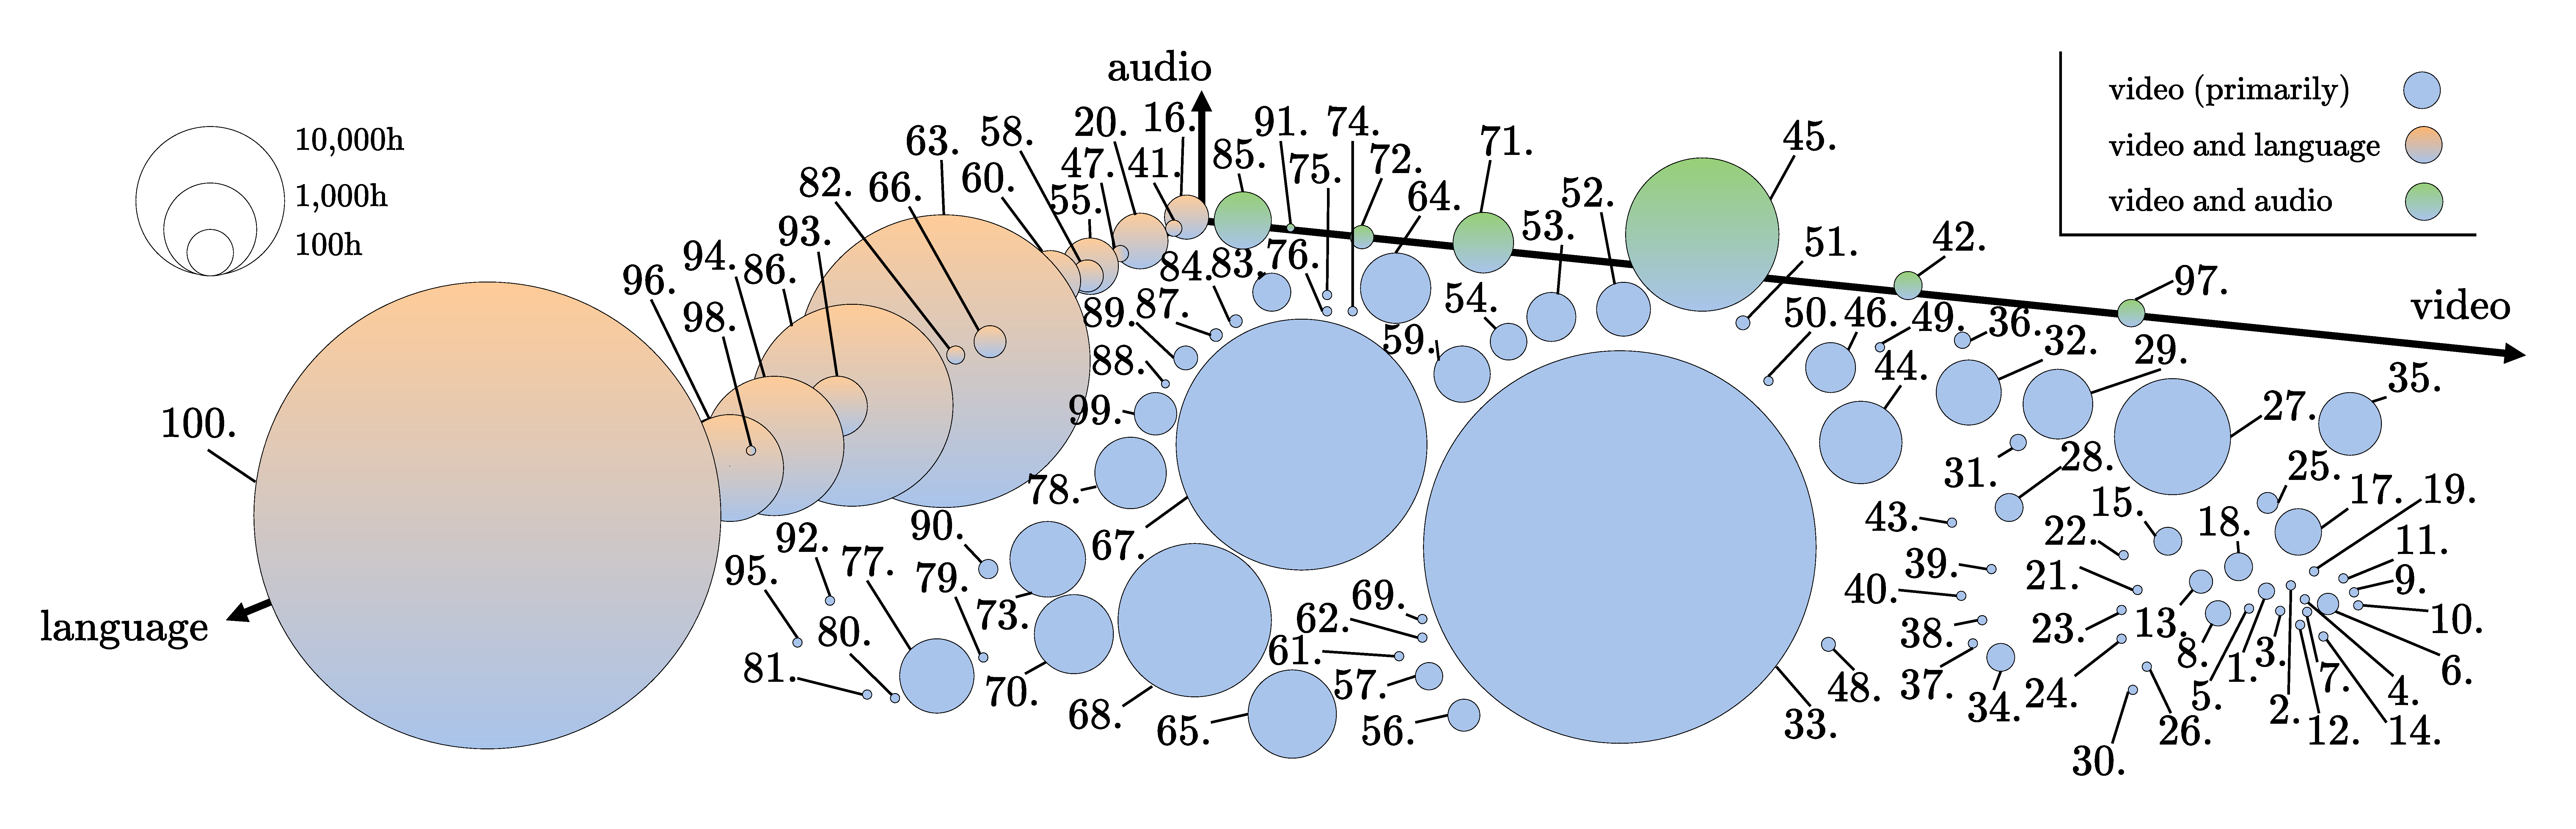
\includegraphics[width=\linewidth]{figs/datasets.pdf}
    \resizebox{\linewidth}{!}{
    \begin{tabular}{llll}
      1. KTH~\citep{schuldt2004recognizing} &  
      2. Weizmann~\citep{gorelick2007actions} &  
      3. Coffee \& Cigarettes~\citep{laptev2007retrieving} & 
      4. CASIA Action~\citep{wang2007human} \\ 
      5. UCF Sports~\citep{rodriguez2008action} & 
      6. Hollywood~\citep{laptev2008learning} & 
      7. UT-Interaction~\citep{ryoo2009spatio} & 
      8. CMU-MMAC~\citep{deguide2008guide} \\
      9. UCF-11~\citep{liu2009recognizing} & 
      10. Hollywood2~\citep{marszalek2009actions} & 
      11. TV-HI~\citep{patron2010high} &
      12. Humaneva~\citet{sigal2010humaneva} \\
      13. UCF-50~\citep{reddy2013recognizing} & 
      14. Olympic Sports~\citep{niebles2010modeling} &
      15. HMDB-51~\citep{kuehne2011hmdb} &
      16. MSVD~\citep{chen2011collecting} \\
      17. CCV~\citep{jiang2011consumer} & 
      18. UCF-101~\citep{soomro2012ucf101} &
      19. CAD-60~\citep{sung2012unstructured} &
      20. MPII~\citep{rohrbach2012database} \\ 
      21. ADL~\citep{pirsiavash2012detecting} &
      22. 50 Salads~\citep{stein2013combining} &
      23. AVENUE~\citep{lu2013abnormal} &
      24. J-HMDB~\citep{jhuang2013towards} \\
      25. CAD-120~\citep{koppula2013learning} &
      26. Penn Action~\citep{zhang2013actemes} &
      27. Sports-1M~\citep{karpathy2014large} & 
      28. EGTEA Gaze+~\citep{li2015delving} \\
      29. ActivityNet-100~\citep{caba2015activitynet} &
      30. Watch-n-Patch~\citep{wu2015watch} &
      31. NTU-RGB-60~\citep{shahroudy2016ntu} &
      32. ActivityNet-200~\citep{caba2015activitynet} \\
      33. YouTube-8M~\citep{abu2016youtube} &
      34. Charades~\citep{sigurdsson2016hollywood} &
      35. ShakeFive2~\citep{van2016spatio} &
      36. DALY~\citep{weinzaepfel2016towards} \\
      37. OA~\citep{li2016recognition} &
      38. CONVERSE~\citep{edwards2016pose} &
      39. TV-servies~\citep{de2016online} & 
      40. Volleyball~\citep{ibrahim2016hierarchical} \\
      41. MSR-VTT~\citep{xu2016msr} &
      42. Greatest Hits~\citep{owens2016visually} &
      43. Okutama Action~\citep{barekatain2017okutama} &
      44. K-400~\citep{kay2017kinetics} \\
      45. AudioSet~\citep{gemmeke2017audio} &
      46. Smthng-Smthng (v1/v2)~\citep{goyal2017something} &
      47. TGIF~\citep{jang2017tgif} &
      48. CMU Panoptic~\citep{joo2017panoptic} \\
      49. MultiTHUMOS~\citep{yeung2018every} &  
      50. RESOUND~\citep{li2018resound} &
      51. EK-55~\citep{damen2018scaling} &
      52. K-600~\citep{carreira2018short} \\
      53. VLOG~\citep{fouhey2018lifestyle} &
      54. AVA~\citep{gu2018ava} &
      55. TVQA~\citep{lei2018tvqa} &
      56. UCF-Crime~\citep{sultani2018real} \\
      57. Charades-Ego~\citep{sigurdsson2018charades} &
      58. YouCook2~\citep{zhou2018towards} &
      59. K-700~\citep{carreira2019short} &
      60. COIN~\citep{tang2019coin} \\
      61. AIST~\citep{tsuchida2019aist} &
      62. Drive\&act~\citep{martin2019drive} &
      63. HowTo100m~\citep{miech2019howto100m}&
      64. Moments in Time~\citep{monfort2019moments} \\
      65. HACS~\citep{zhao2019hacs} &
      66. VATEX~\citep{wang2019vatex} &
      67. IG65M~\citep{ghadiyaram2019large} &
      68. Toyota Smarthome~\citep{dai2022toyota} \\
      69. OOPS~\citep{epstein2020oops} &
      70. AViD~\citep{piergiovanni2020avid} &
      71. VGGSound~\citep{chen2020vggsound} &
      72. LLP~\citep{tian2020unified} \\
      73. HVU~\citep{diba2020large} &
      74. DMP~\citet{ortega2020dmd} &
      75. Action Genome~\citep{ji2020action} &
      76. Countix~\citep{dwibedi2020counting} \\
      77. K-700 (2020)~\citep{smaira2020short} &
      78. FineGym~\citep{shao2020finegym} & 
      79. RareAct~\citep{miech2020rareact} &
      80. Immersive Light Field~\citet{broxton2020immersive} \\
      81. HAA500 \citep{chung2021haa500} &
      82. IKEA ASM~\citep{ben2021ikea} &
      83. MultiSports~\citep{li2021multisports} &
      84. MOMA~\citep{luo2021moma} \\
      85. Spoken Moments~\citep{monfort2021spoken} &
      86. WebVid-2M~\citep{bain2021frozen} &
      87. Home action genome~\citep{rai2021home} & 
      88. DanceTrack~\citep{sun2022dancetrack} \\
      89. EK-101~\citep{damen2022rescaling} &
      90. FineAction~\citep{liu2022fineaction} &
      91. AVSBench~\citep{zhou2022audio} &
      92. Neural 3D Video~\citet{li2022neural} \\
      93. Assembly101~\citep{sener2022assembly101} &
      94. Ego4D \citep{grauman2022ego4d} &
      95. SportsMOT~\citep{cui2023sportsmot} &
      96. Ego-Exo-4D \citep{grauman2024ego} \\ 
      97. EPIC-Sounds \citep{huh2023epic} &
      98. MVBench \citep{li2024mvbench} &
      99. OVR \citep{dwibedi2024ovr} &
      100. Vidchapters-7M \citep{yang2024vidchapters}
    \end{tabular}
    }
    \caption{\textbf{Datasets compared by total dataset duration and primary modality}. Circle sizes correspond to the (approximate) summed duration of all videos in the datasets. Recent datasets (i.e., $>80$) have longer total running times and include additional modalities such as language or audio.}
    \label{fig:dataset_blobs}
\end{figure*}

\subsection{Data collection challenges}
\label{sec:datasets::challenges}

\noindent
\textbf{Ensuring sufficient diversity} of people, scenarios, and activities is important when amassing video datasets at scale. Although in recent years scalability has been achieved by transiting from locally-sourced datasets \pcite{caba2015activitynet,laptev2008learning,shahroudy2016ntu,schuldt2004recognizing,soomro2012ucf101} to multi-team-multi-year efforts \pcite{grauman2022ego4d,li2024mvbench,yang2024vidchapters} dataset diversity remains subjective which can result to semantically overlapping \pcite{khamis2015walking,wray2019learning} or ambiguous \pcite{kim2022action,sigurdsson2017actions} labels. As video understanding is a multifaceted topic relating to vision, robotics, and augmented reality, collecting \textbf{meaningful scenarios and annotations} also presents difficulties. Several datasets have used surveys \pcite{caba2015activitynet,grauman2022ego4d,grauman2024ego,lin2023videoxum} or relied on meta-data from online videos \pcite{chen2023vast,miech2019howto100m,smaira2020short,yang2024vidchapters} as guides for collection. Despite such efforts, sourcing is still bound to preliminary data assumptions \pcite{rahaman2022generalized}, inconsistencies across annotations \pcite{moltisanti2017trespassing}, and difficulties in task definitions \pcite{alwassel2018diagnosing}. The collection pipelines also require scalability. In recency, \textbf{greater automation} in video collection has been achieved with the use of embeddings from vision encoders \pcite{chen2020vggsound,huang2024vbench,zhu2024video}, and LLM-generated descriptions \pcite{fu2024video,li2024videovista,mangalam2023egoschema}.



\subsection{General datasets}
\label{sec:datasets::general}

The past two decades have seen a significant increase in dataset size, leading to more robust baselines. We present widely-adopted benchmarks chronologically in \Cref{tab:action_recognition_datasets}. The primary focus of initial benchmarks \pcite{schuldt2004recognizing,gorelick2007actions} has been the categorization of simple actions such as \emph{walking} and \emph{hand waving}. Subsequent datasets predominantly comprised videos from either TV shows/movies \pcite{laptev2007retrieving,laptev2008learning,marszalek2009actions,patron2010high,kuehne2011hmdb} or sports footage \pcite{rodriguez2008action,liu2009recognizing,reddy2013recognizing,niebles2010modeling}. Important steps towards establishing large-scale datasets for the video domain were made with the introduction of Sports-1M \pcite{karpathy2014large}, YouTube-8M \pcite{abu2016youtube}, and Kinetics \pcite{carreira2017quo} that include web-sourced videos of a diverse range of actions. Evident from their sizes shown in \Cref{fig:dataset_blobs}, these datasets paved the way as general benchmarks for models that can subsequently be adapted to smaller, more niche datasets such as UCF-101 \pcite{soomro2012ucf101} and ActivityNet \pcite{caba2015activitynet}. Despite their size and use in multiple downstream tasks, there is still room to address specific action understanding tasks or modalities supplementary to vision. Domains such as 
egocentric vision, human-object interaction recognition, and hierarchical action understanding have gained popularity, prompting the creation of domain-specific datasets. EGTEA Gaze+ \pcite{li2015delving}, EPIC KITCHENS \pcite{damen2022rescaling}, and later EGO4D \pcite{grauman2022ego4d} have been the main benchmarks for egocentric vision. Something-Something \pcite{goyal2017something} and Charades \pcite{sigurdsson2016hollywood} have been predominantly used as benchmarks for object-based actions with a greater focus on temporal information. Datasets such as Diving-48 \pcite{li2018resound} and FineGym \pcite{shao2020finegym} incorporate semantic hierarchies in their annotations. More recent datasets have focused on tasks related to action recognition including instruction learning \pcite{alayrac2016unsupervised,bansal2022my,ben2021ikea,liui2024kea,ohkawa2023assemblyhands,sener2022assembly101,tang2019coin}, action phase alignment \pcite{sermanet2017unsupervised}, repeating action counting \pcite{dwibedi2020counting,dwibedi2024ovr,hu2022transrac,runia2018real,zhang2020context}, action completion prediction \pcite{epstein2020oops}, driver behavior recognition \pcite{martin2019drive,ortega2020dmd}, anomaly detection \pcite{acsintoae2022ubnormal,liu2018future,lu2013abnormal,sultani2018real,wu2020not}, hand-object interactions \pcite{chao2021dexycb,garcia2018first,hampali2020honnotate,kwon2021h2o,moon2020interhand2,mueller2017real}, and object state change detection in actions \pcite{souvcek2022look}. 



\subsection{Domain- and modality-specific datasets}
\label{sec:datasets::specific}

Apart from general-purpose datasets, several benchmarks have been designed to evaluate model capabilities of specific aspects of action understanding. We overview of benchmarks in three groups: based on the holistic understanding of scenes from multiple viewpoints, and with supplementary modalities such as language and audio.

% Multi-view and multi-camera set-ups
\noindent
\textbf{Multi-view}. Initial efforts to compile multi-view videos included a small number of subjects \pcite{sigal2010humaneva} or synthetic data \pcite{ionescu2013human3}. High-quality multi-view videos depend highly on the hardware and setup \pcite{wang2023learning}. CMU panoptic \pcite{joo2017panoptic} captured group interactions within a dome with 480 cameras. Interactions included social settings, games, dancing, and musical performances. ZJU-Mocap \pcite{peng2021neural} comprised dynamic videos of human motions from 20 cameras. The Immersive Light Field dataset \pcite{broxton2020immersive} contains videos with 6 degrees of freedom from a camera rig consisting of 46 action cameras. Multi-view datasets are collected for a variety of target tasks, including dance sequence reconstruction \pcite{tsuchida2019aist}, and the dynamic synthesis of indoor spaces in which actions take place \pcite{dai2022toyota,tschernezki2024epic}.

% 3D
\noindent
\textbf{3D vision}. 3D human action reconstruction initially relied on synthetic data \pcite{anguelov2005scape,bronstein2010shrec} or lacked detailed ground-truth annotations \pcite{koppula2013learning,li2010action,shahroudy2016ntu,sung2012unstructured}. (D)FAUST \pcite{bogo2014faust,bogo2017dynamic} introduced a full pipeline for capturing high-resolution deformations. The collected 3D models of 300 meshes from static scans later increased to 40K meshes from dynamic scans. With the same multi-camera setting, DYNA \pcite{pons2015dyna} collected meshes by aligning 3D scans to template meshes using only geometric information. Other 3D data collection efforts have been specific to action synthesis in indoor \pcite{li2022neural} and outdoor \pcite{lin2021deep,yoon2020novel} settings, depth-based procedural learning \pcite{ben2021ikea,sener2022assembly101}, human-object interaction tracking \pcite{bhatnagar2022behave}, novel view synthesis \pcite{jiang2022neuman,peng2021neural}, language captioning for poses \pcite{delmas2022posescript}, or representing human-relevant attributes such as clothes and hair dynamics \pcite{black2023bedlam}. Large-scale collections that unify existing datasets also exist. \tcite{guo2020action2motion} created a dataset for 3D human motions by revamping \tcite{joo2017panoptic,shahroudy2016ntu,zou20203d}. Similarly,  \tcite{mahmood2019amass} combined a corpus of 15 archival marker-based mocap datasets while \tcite{lin2023motion} created a superset of datasets by sourcing videos \pcite{cai2022humman,chung2021haa500,taheri2020grab,tsuchida2019aist,zhang2022egobody} relevant to LLM motion text prompts. Recently, space-time-depth datasets and benchmarks have also been introduced for egocentric data for tracking human-object interactions \pcite{liu2022hoi4d,perrett2025hd}, mistake detection in procedural tasks \pcite{wang2023holoassist}, multi-task augmented reality \pcite{grauman2024ego,lv2024aria,pan2023aria}, and surface estimation and reconstruction \pcite{straub2024efm3d}.

% Language-related datasets
\noindent
\textbf{Video-language}. In recent years, language has been integrated into vision methods as a natural extension to represent high-level semantics. Commonly, learning to map textual concepts and visual representations in a shared embedding space has been a widely adopted strategy by many video tasks \pcite{amrani2021noise,gabeur2020multi,liu2019use,miech2020end}. Initial video-language datasets \pcite{chen2011collecting,xu2016msr} were based on short video snippets and short textual descriptions of actions. More recent efforts also provide multilingual descriptions \pcite{wang2019vatex}. Video question-answering is a popular language-based task \pcite{jang2017tgif,lei2018tvqa,li2024mvbench,oncescu2021queryd,rawal2024cinepile,xiao2021next}. The order of instructions has been of great interest in longer videos since the introduction of HowTo100M \pcite{miech2019howto100m} and YouCook2 \pcite{zhou2018towards}. Benchmarks have also been proposed for other long-form tasks such as moment retrieval \pcite{rohrbach2015dataset,song2024moviechat,yang2024vidchapters}, frame extraction \pcite{li2024llava}, multimodal open-ended question answering \pcite{fu2024video,ying2024mmt}, and long-term reasoning \pcite{chandrasegaran2024hourvideo,fei2024video,mangalam2023egoschema}.

% Video and audio
\noindent
\textbf{Audio and vision}. Human perception often relies on the inclusion of audio for understanding actions, especially in conditions where appearance may lead to ambiguous predictions. Audioset \pcite{gemmeke2017audio} is the largest audio-visual action dataset containing 2.1M clips across a long-tail distribution of 527 classes. VGG-Sound \pcite{chen2020vggsound} is another common benchmark with a uniform distribution of 200K videos over 300 classes. Datasets have also been collected for specific tasks such as audio-visual semantic segmentation \pcite{zhou2022audio}, audio-visual video parsing \pcite{tian2020unified}, material sound and action classification \pcite{huh2023epic,owens2016visually}, and video captioning \pcite{monfort2021spoken}.

% link to next section
The introduction of both general and task-specific datasets has improved the exploration of video tasks and standardized evaluation protocols. Main lines of research and challenges of these tasks are overviewed next.